\chapter{Implementation}

\section{Development Process}

\subsection{Initial Architecture Design}

The development process began with a modular architecture centered on four primary components. The Camera Control System is responsible for managing all interactions with the camera and overseeing image capture. Dataset Management ensures data persistence and organization, handling the storage and categorization of captured images and their metadata. The Analysis Engine processes these images to perform lens measurements, such as evaluating sharpness and vignetting. Finally, the User Interface allows users to interact with the application, configuring settings and visualizing results.

\subsection{Camera Integration Development}

The integration of the camera system was approached in three phases.

In Phase 1, Basic Camera Communication, we integrated the gphoto2 library to facilitate camera control. We implemented basic logic for connecting and disconnecting the camera and developed a system to monitor the camera's status. Basic error handling and recovery mechanisms were also established to manage initial connection issues.

Phase 2 focused on Advanced Camera Control. In this phase, we comprehensively managed camera settings, including manual and auto-focus controls. We added capabilities for capturing images in RAW format and implemented real-time monitoring of the camera's status to provide immediate feedback on its operation.

In Phase 3, the emphasis was on Robustness Improvements. We made camera operations thread-safe to prevent concurrent access issues. We implemented automatic reconnection handling to maintain camera connectivity and optimized memory management to efficiently handle image capture processes. Additionally, we introduced timeout handling to manage prolonged camera operations gracefully.

\subsection{Analysis Engine Development}

The Analysis Engine's development progressed through three stages.

Stage 1, Core Analysis Functions, involved implementing the raw image processing pipeline, including algorithms for calculating the Modulation Transfer Function (MTF) and performing edge detection and basic lens distortion measurements.

In Stage 2, Advanced Analysis Features were introduced, enhancing the engine with capabilities such as bokeh quality analysis, chromatic aberration detection, vignetting measurement, and generating visualizations of analysis results.

Stage 3 focused on Optimization, where we improved the processing of large images, optimized memory usage, refined the accuracy of analysis algorithms, and added support for multi-threaded analysis to increase processing efficiency.

\subsection{Data Management Implementation}

The Data Management system was developed in two phases.

During the Core Functionality phase, we established the dataset creation and storage system, organized files hierarchically, managed comprehensive metadata, and implemented storage for analysis results.

In the Advanced Features phase, we added functionalities for importing and exporting datasets, managing structured scenarios, comparing analysis results, and verifying data integrity to ensure the reliability of stored information.

\subsection{Integration and Testing}

The integration process concentrated on two main areas: Component Integration and Testing Procedures.

In Component Integration, we systematically integrated the core components, ensuring that interfaces between different modules were compatible. We optimized performance and verified resource management to ensure efficient operation.

Testing Procedures involved conducting comprehensive unit tests, performing integration tests to ensure components worked together seamlessly, executing performance load tests to assess the system's handling of high data volumes, and verifying the functionality of the user interface.

\subsection{Deployment Considerations}

The final phase addressed deployment requirements, focusing on System Requirements and Documentation.

For System Requirements, we conducted hardware compatibility testing, managed dependencies, developed the installation process, and managed system configuration to ensure the application could be reliably deployed.

In terms of Documentation, we created technical documentation, user guides, API documentation, and installation guides to support users and developers in understanding and utilizing the application effectively.

\section{Used Technologies}

\subsection{Dependencies}

The project is built using the Python programming language and leverages several Python libraries and tools. The gphoto2 library is utilized for core camera communication and control, enabling interaction with various camera models. OpenCV provides robust image processing and analysis capabilities essential for the Analysis Engine. NumPy is employed for numerical computations and array operations, facilitating efficient data handling. Rawpy is used for processing RAW image files, ensuring high-quality image data is available for analysis. NiceGUI serves as the web-based user interface framework, allowing for the creation of an interactive and user-friendly interface.

\subsection{Development Environment}

The development environment integrates various tools and configurations to support efficient and organized software development. Git is used for version control, enabling us to track code changes and collaborate effectively. The primary platform for development is Linux, chosen for its robustness and versatility. Python virtual environments are employed to isolate dependencies, ensuring a clean and consistent development setup. Additionally, an automated testing framework is incorporated to streamline testing processes, validate functionality, and maintain code quality throughout the development lifecycle.

\section{Implementation of System Components}

\subsection{Camera Control System}

The Camera Control System is implemented within the \texttt{CameraManager} class, utilizing the gphoto2 Python library. The \texttt{CameraManager} initializes the camera context and establishes a connection using thread-safe locks to ensure safe concurrent operations. It continuously monitors the camera's connection status, managing reconnections as needed to maintain robust operation.

Key features include listing all available camera properties by recursively exploring the camera's configuration widgets. This allows dynamic adjustments to parameters such as aperture, ISO, shutter speed, and exposure modes. The class also extracts metadata from images by leveraging EXIF data to gather information like focal length, lens type, and exposure settings.

Image capture functionality incorporates autofocus handling and respects existing camera settings. Captured images, along with their metadata, are systematically stored to facilitate subsequent analysis. Comprehensive error handling manages hardware exceptions and unexpected states, such as camera unavailability, by logging detailed error messages and retrying operations when appropriate.

\subsubsection{Camera Control Architecture}

A fundamental architectural decision in the Camera Control System was whether to integrate directly with the gphoto2 library or implement a REST API-based control system. Direct integration was chosen for several reasons. It offers lower latency for camera operations, allowing precise timing for captures and settings changes. Direct access to camera events is crucial for real-time monitoring of camera status and capture completion. Handling large RAW files is more efficient with direct memory access, and direct exception handling provides better control over camera-related errors. Additionally, this approach allows full access to camera features without the limitations of an API abstraction layer.

Although a REST API-based control system provides advantages in terms of scalability and system integration, the performance and control requirements of lens testing necessitated the direct integration approach. To mitigate the tight coupling to gphoto2, the \texttt{CameraManager} class carefully abstracts camera interactions, allowing for potential future adaptations if requirements change.

Here is an example of how image capture is handled within the \texttt{CameraManager} class:

\begin{verbatim}
def capture_image(self):
    try:
        file_path = self.camera.capture(gp.GP_CAPTURE_IMAGE)
        camera_file = self.camera.file_get(
            file_path.folder,
            file_path.name,
            gp.GP_FILE_TYPE_NORMAL
        )
        return camera_file
    except gp.GPhoto2Error as e:
        logging.error(f"Capture failed: {e}")
        raise
\end{verbatim}

And an example of how a REST API-based implementation would look:

\begin{verbatim}
@app.post("/api/camera/capture")
async def capture_image():
    try:
        response = await client.post(
            f"{CAMERA_SERVICE_URL}/capture",
            headers={"Authorization": AUTH_TOKEN}
        )
        if response.status_code == 200:
            return response.json()
        raise HTTPException(status_code=response.status_code)
    except Exception as e:
        raise HTTPException(status_code=500, detail=str(e))
\end{verbatim}

\subsection{Dataset Management}

Managing datasets effectively is crucial for organizing captured images and associated metadata. Two architectural approaches were considered: centralized server-side management and split browser-server management.

Centralized Server-Side Management maintains all dataset management on the server, including both metadata and RAW files. This approach offers several advantages. It ensures strong data consistency with a single source of truth, simplifies transaction management for dataset operations, and reduces complexity in maintaining data synchronization. It is also better suited for multi-user scenarios and facilitates easier backup and version control of complete datasets. However, this approach has its disadvantages, such as higher server resource utilization, increased network traffic for metadata operations, potential latency in UI operations, and a less responsive interface for dataset organization.

On the other hand, Split Browser-Server Management divides responsibilities by handling metadata management in the browser while RAW files remain on the server. This leads to a more responsive user interface for dataset operations, reduces server load for metadata tasks, and lowers bandwidth usage for organizational activities. Additionally, it enhances offline capabilities for dataset organization and allows faster sorting and filtering of datasets. On the downside, this approach introduces more complex data synchronization requirements, potential consistency issues between client and server, and adds complexity in handling multi-user scenarios. It also complicates error recovery and necessitates conflict resolution in metadata.

\subsection{Technical Considerations}

Several technical aspects were considered when evaluating these approaches, including data storage, network usage, scalability, implementation complexity, and error handling. Centralized management involves managing all data in the server filesystem and database, resulting in higher network usage for metadata operations but consistent handling for RAW files. It is limited by server resources and has lower implementation complexity, being a straightforward Python implementation. Error handling is simpler, with easier recovery from failures.

In contrast, split management stores RAW files on the server and metadata in browser storage, resulting in lower network usage for metadata but the same for RAW files. It offers better scalability through distributed computational load but has higher implementation complexity due to the need for browser-server synchronization. Error handling is more complex, requiring more sophisticated state management.

\begin{table}[h]
\centering
\begin{tabular}{|p{3cm}|p{5cm}|p{5cm}|}
\hline
\textbf{Aspect} & \textbf{Centralized} & \textbf{Split Management} \\
\hline
Data Storage & All data managed in server filesystem and database & RAW files on server, metadata in browser storage \\
\hline
Network Usage & Higher for metadata operations, consistent for RAW files & Lower for metadata, same for RAW files \\
\hline
Scalability & Limited by server resources & Better distribution of computational load \\
\hline
Implementation Complexity & Lower, straightforward Python implementation & Higher, requires browser-server synchronization \\
\hline
Error Handling & Simpler recovery from failures & More complex state management required \\
\hline
\end{tabular}
\caption{Technical Comparison of Dataset Management Approaches}
\label{table:dataset_comparison}
\end{table}

\subsection{Selected Approach}

For this implementation, the centralized server-side management approach was chosen for several key reasons. The critical nature of lens testing data requires strong consistency guarantees, which are best provided by a single source of truth. The simpler architecture allows for faster development and testing, adhering to the project's implementation timeline. Additionally, this approach provides a better foundation for future expandability, such as adding multi-user support and version control. Maintaining data integrity is easier with centralized management, as it simplifies referential integrity between metadata and RAW files. Moreover, error recovery is more straightforward, with simpler backup and recovery procedures.

While the split browser-server model offers advantages in UI responsiveness and resource distribution, the added complexity and potential consistency issues were deemed to outweigh these benefits for the current scope of the application. However, the architecture remains modular enough that transitioning to a split model could be implemented in future versions if requirements change.

The selected architecture aligns well with the project's primary goals of reliability and accuracy in lens testing, maintaining a balance between implementation complexity and system robustness.

\section{Analysis Engine}

\subsection{Preprocessing vs. Processing}

A key part of the image analysis workflow is distinguishing between **preprocessing** and **processing** steps. These two phases serve distinct purposes and occur at different points in the workflow.

**Preprocessing** includes all operations that are uniform and necessary before an image enters scenario-specific analysis. The goal is to ensure that every input photograph, regardless of its eventual analytical purpose, is brought to a consistent baseline. This involves tasks such as converting RAW images to a standard format like TIFF or PNG, applying lens corrections that are independent of specific scenarios, normalizing image brightness or contrast to account for variations in lighting and camera settings, and removing sensor noise or unwanted digital artifacts common to all captures. By performing these steps upfront, the system ensures that downstream processes operate on images with a predictable level of quality, uniformity, and formatting. Preprocessing is scenario-agnostic and solely focused on preparing the inputs consistently.

**Processing**, in contrast, refers to the suite of analyses and transformations that depend on the specific scenario at hand. For example, if the analysis is focused on evaluating sharpness, the processing stage might involve localizing test-chart features, computing sharpness metrics, and extracting spatial frequency responses. If the scenario is centered on vignetting, processing might involve measuring the illumination fall-off towards the corners and computing vignetting scores. These operations are scenario-specific, requiring knowledge of the particular tests being run, the metrics to be derived, and the structures or patterns expected in the images.

In summary, **preprocessing** consists of universal, scenario-independent steps applied to every photo to ensure consistent starting conditions, while **processing** involves scenario-specific analysis steps that derive particular measurements, scores, or insights from the image based on the experiment’s goals.

\subsection{Image Preprocessing and Segmentation}

The image processing pipeline begins with an initial segmentation phase that identifies calibration elements within the image. Utilizing algorithms such as SIFT, the pipeline detects and localizes key graphical features of the test charts. This step lays the groundwork for subsequent stages by eliminating irrelevant areas of the image.

Following segmentation, preprocessing applies a series of transformations to normalize the data. Preprocessing tasks include noise reduction, image resizing, and contrast adjustment to account for variations in lighting and camera settings. The application of median or Gaussian filters ensures that these transformations preserve critical details. Additionally, the pipeline converts raw image data into an analyzable format, setting the stage for accurate and reliable analysis.

\subsection{Feature Detection and Analysis}

The next stage involves evaluating specific lens properties. For sharpness analysis, edge detection techniques are employed to assess transitions between high-contrast regions. The modulation transfer function (MTF) is calculated to quantify spatial resolution, providing a robust measure of lens clarity. Vignetting is assessed by analyzing the intensity distribution across the image, while geometric distortion is evaluated by comparing expected grid patterns to their actual appearance. Chromatic aberrations are quantified by measuring color fringing at the boundaries of high-contrast features, and bokeh quality is examined by characterizing out-of-focus light regions.

A key characteristic of the pipeline is its adaptability to various calibration test charts and environmental conditions. This is achieved through parameterized algorithms and automated calibration routines. The pipeline also integrates mechanisms to validate the reliability of the extracted data, detecting and discarding outliers that might result from erroneous inputs.

Processed data is formatted for visualization and reporting, with analytical results structured into metrics and graphs. These results are also stored for future reference, ensuring that comprehensive records of lens performance are maintained.

\section{User Interface Components}

\subsection{Camera Control Panel}

The camera control panel offers a centralized interface for managing camera operations. Users can easily connect and disconnect the camera, with real-time monitoring of the camera’s status. Advanced camera controls allow access to settings such as aperture, shutter speed, and ISO. The application supports both automatic and manual focus adjustments, providing flexibility for various testing scenarios. Additional functionalities include capturing images directly through the interface, importing RAW files, and listing all available camera properties.

\begin{figure}[h]
\centering
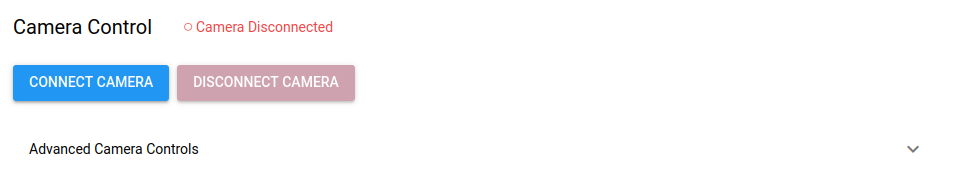
\includegraphics[width=1\textwidth]{Images/camera_control.png}
\caption{Camera control panel.}
\label{fig:ui_camera_control}
\end{figure}

\subsection{Datasets Panel}

The datasets panel enables users to handle captured images and related metadata efficiently. Users can import, create, select, and manage datasets, ensuring systematic storage and categorization of images. Each image is linked to a specific scenario, allowing users to structure their tests based on various lens properties. Metadata embedding ensures that all relevant information, including camera settings and capture details, is preserved for future reference. The system supports structured file naming conventions and temporary storage management, ensuring consistency and ease of navigation.

\begin{figure}[h]
\centering
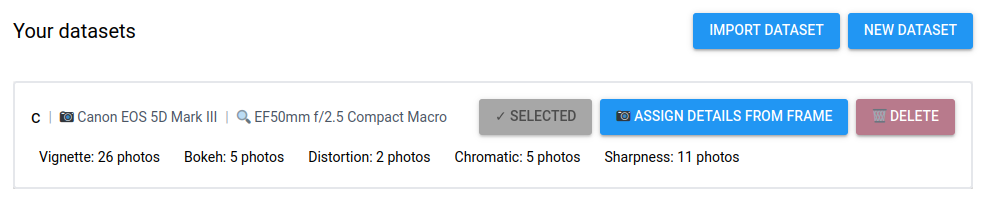
\includegraphics[width=1\textwidth]{Images/datasets_panel.png}
\caption{Datasets panel.}
\label{fig:ui_datasets}
\end{figure}

\subsection{Scenarios Panel}

The scenarios panel allows users to target lens evaluations to specific properties, such as sharpness, vignetting, distortion, chromatic aberrations, and bokeh. Each scenario is linked to a dataset and includes predefined settings and workflows for capturing and analyzing images.

\begin{figure}[hbt]
\centering
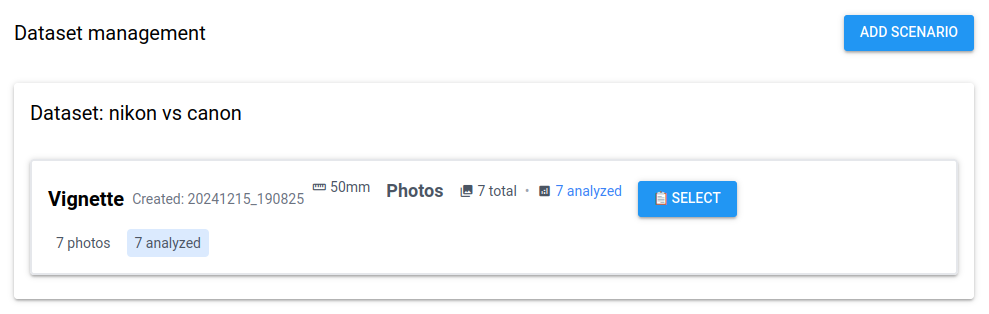
\includegraphics[width=1\textwidth]{Images/scenarios_panel.png}
\caption{Scenarios panel.}
\label{fig:ui_scenarios}
\end{figure}

\subsection{Analysis Results}

Users can view detailed analysis results presented in a structured format. The Capture Settings section at the top summarizes the camera configuration during image capture, including details such as the camera model, lens information, aperture setting, shutter speed, ISO sensitivity, and focal length. These settings provide context for understanding the conditions under which the analysis was performed.

\begin{figure}[hbt]
\centering
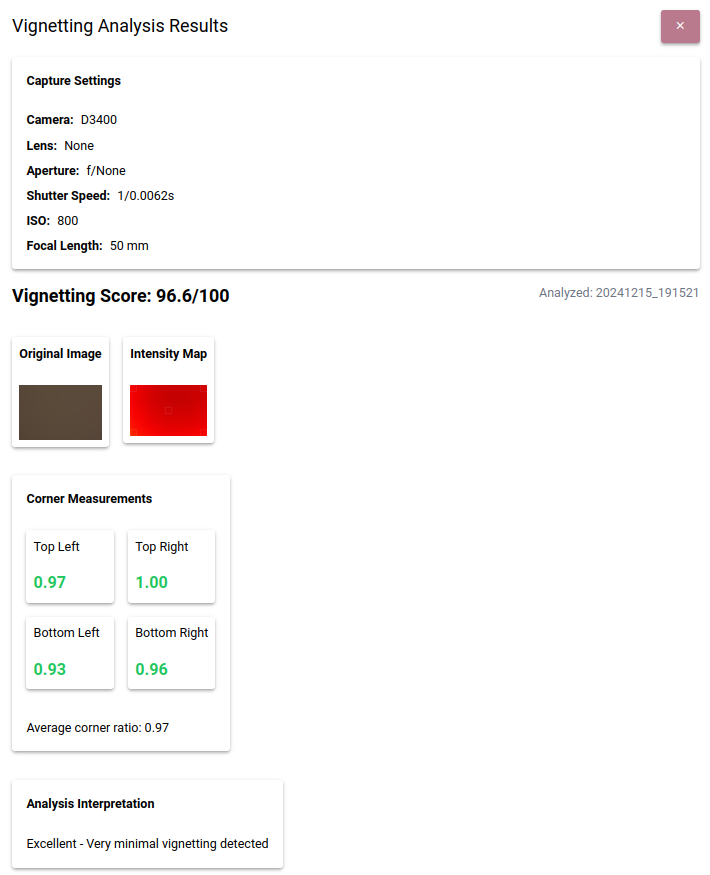
\includegraphics[height=0.8\textwidth]{Images/scenario_result.png}
\caption{Result of vignette scenario.}
\label{fig:ui_scenario_result}
\end{figure}

The Numerical Scores section offers a quantitative assessment tailored to the specific scenario. For example, in sharpness analysis, this may include metrics like Modulation Transfer Function (MTF) scores. These scores are often normalized to a scale (e.g., 0-100) to simplify interpretation and enable comparisons across different lenses and settings.

The Visual Outputs section includes graphical representations to enhance the understanding of the analysis results. This may involve displaying the original captured image alongside processed visualizations, such as heatmaps, intensity maps, and edge overlays.

The Measurement Details section provides more granular insights, which could include corner measurements for luminance ratios in vignetting analysis or edge intensity values for sharpness.

Finally, the Analysis Interpretation section summarizes the findings in plain language, offering a qualitative assessment of the results. For example, it may indicate whether vignetting is minimal, sharpness is excellent, or distortions are significant. This summary helps users quickly grasp the outcome of the analysis without needing to interpret the raw data or metrics.

\subsection{Analysis Details}

The section with visual outputs and measurement details varies based on the selected analysis type:

In \textbf{Vignetting} analysis, results include center-to-corner luminance ratios, average corner intensity, and a normalized vignetting score. Heatmaps visually represent brightness variations across the image, offering further insights into the vignetting effect.

\begin{figure}[hbt]
\centering
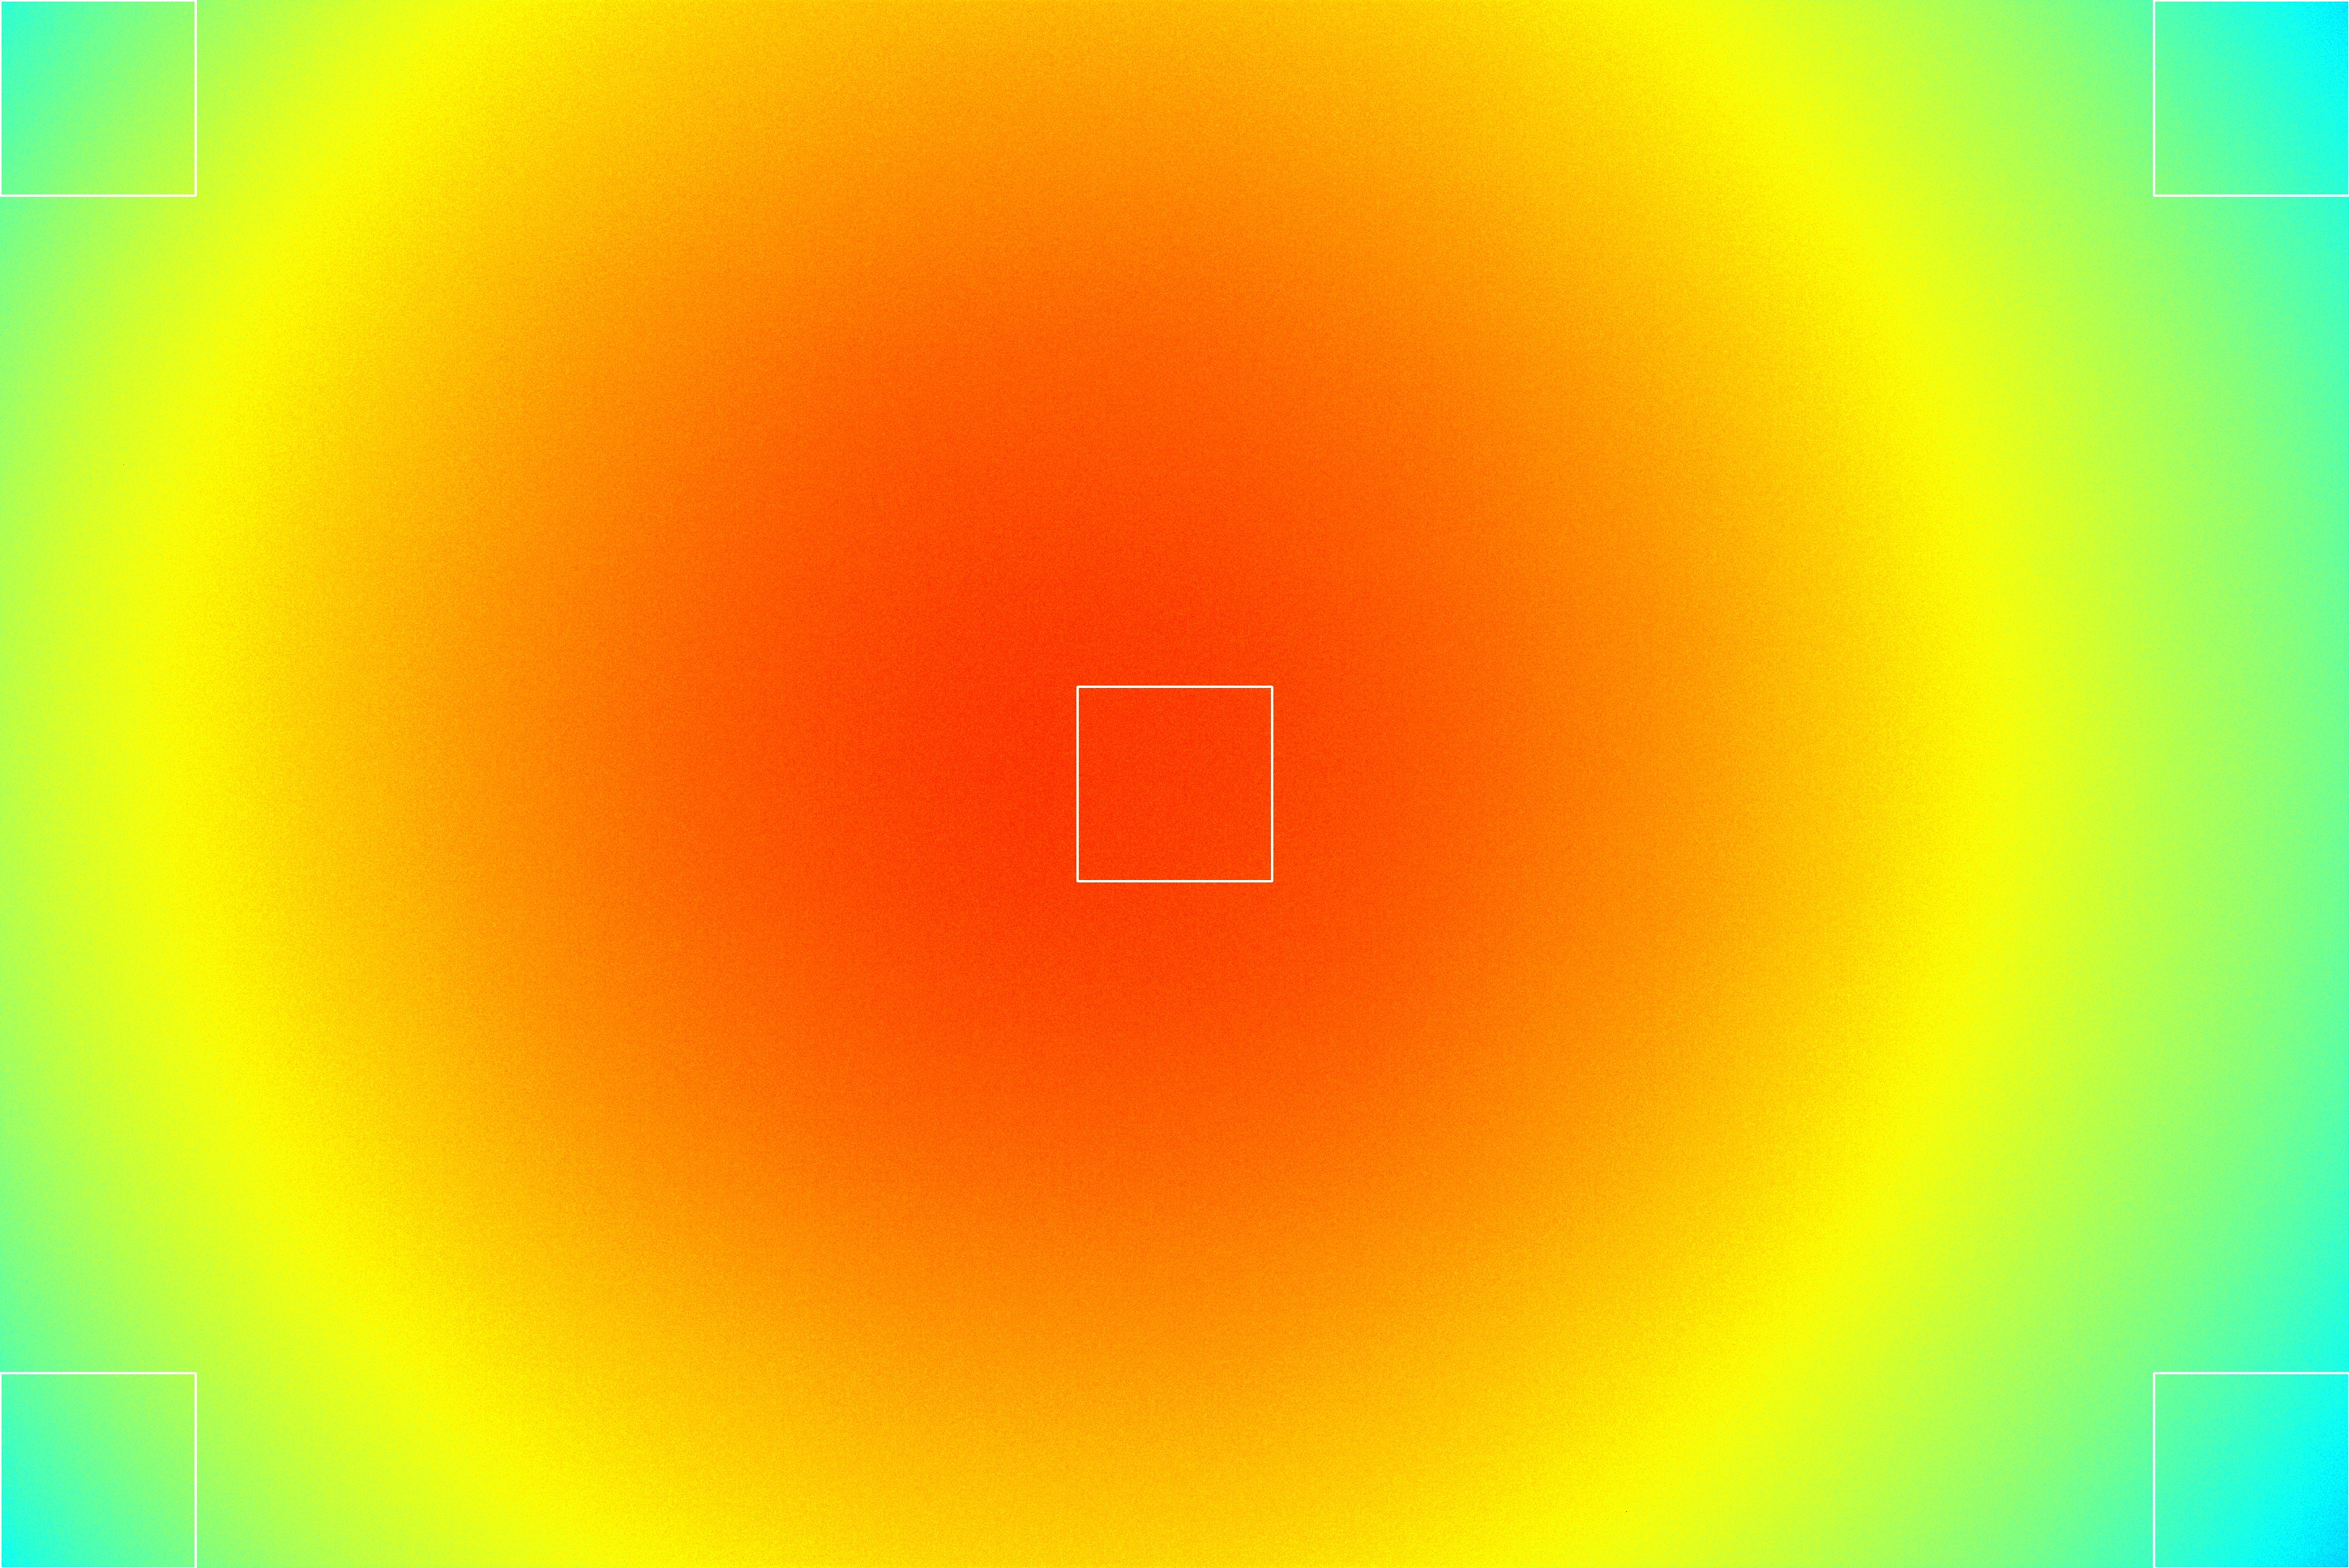
\includegraphics[width=0.6\textwidth]{Images/vignette_image_result.jpg}
\caption{Intensity map for vignette scenario.}
\label{fig:ui_vignette_intensity_map}
\end{figure}

For \textbf{Sharpness} analysis, the UI displays numerical metrics such as Modulation Transfer Function (MTF) scores, edge intensity, and an overall sharpness rating. These are accompanied by graphs illustrating MTF curves across spatial frequencies and edge detection overlays that highlight areas of detail within the image. Original and processed images are shown side by side, providing clear visual comparisons.

\begin{figure}[h]
\centering
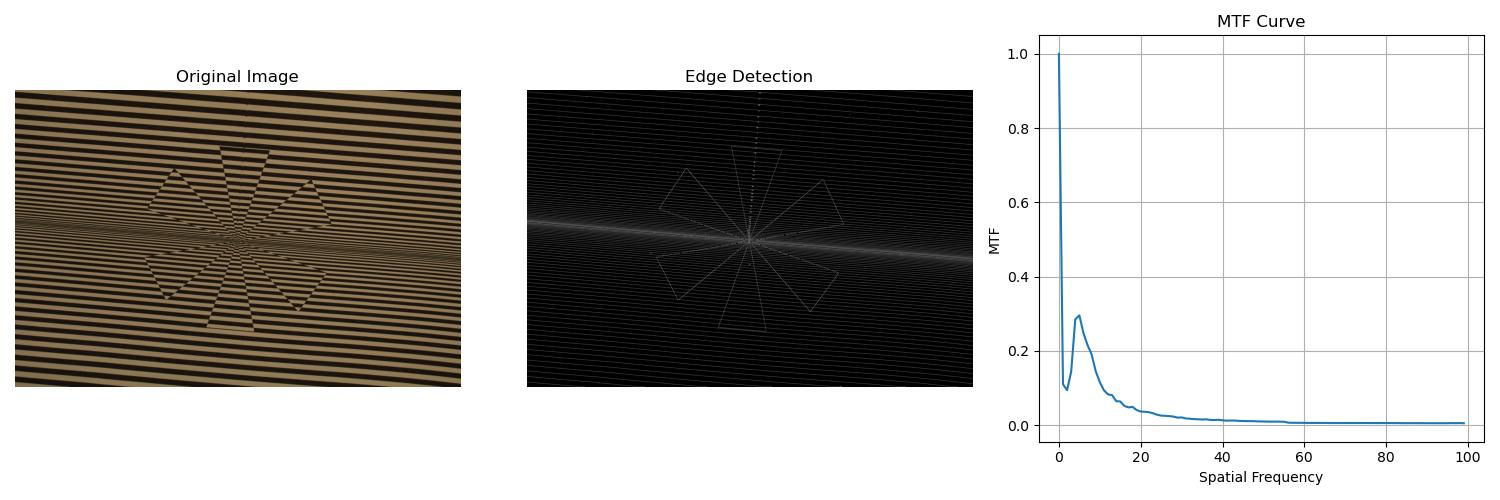
\includegraphics[width=1\textwidth]{Images/sharpness_image_result.jpg}
\caption{Sharpness analysis details.}
\label{fig:ui_sharpness_image}
\end{figure}

In \textbf{Distortion} analysis, the system outputs metrics such as deviations in line straightness, average line deviation, and an overall distortion score. Grid overlays on the original image demonstrate detected distortion patterns, while corrected and uncorrected versions are displayed for comparison. The type of distortion—barrel, pincushion, or waveform—is identified based on the analysis.

\textbf{Chromatic Aberration} analysis highlights color fringing in images, providing metrics on pixel offsets and scores for lateral and longitudinal aberrations. The UI displays zoomed-in sections of the image where chromatic aberrations occur, with overlaid color error vectors for visualization. Original and corrected images are presented side by side to showcase the impact of corrections.

In \textbf{Bokeh} analysis, the system evaluates characteristics such as roundness, smoothness, and consistency of out-of-focus highlights. Overlays highlight bokeh regions, accompanied by metrics for size, shape, and edge definition. Users can compare bokeh characteristics across different aperture settings or light sources using dynamic visualization tools.

\begin{figure}[h]
\centering
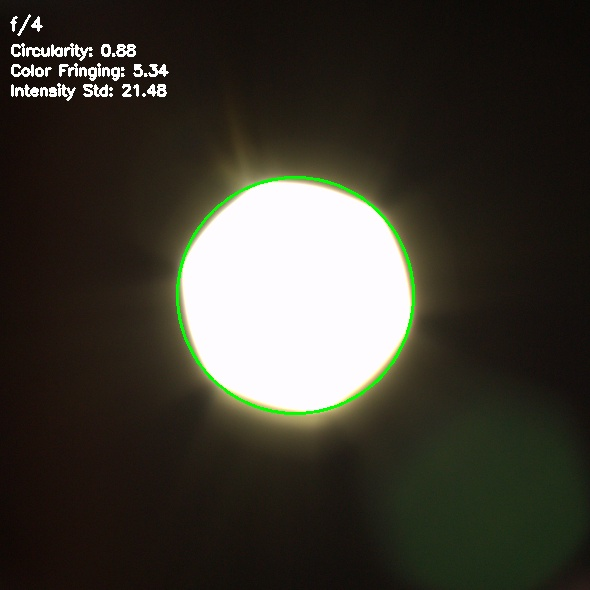
\includegraphics[width=0.35\textwidth]{Images/bokeh_image_result.jpg}
\caption{Bokeh analysis details.}
\label{fig:ui_bokeh_image}
\end{figure}

\subsection{System Logs}

The system logs provide a real-time record of application activities, ensuring transparency and aiding in troubleshooting. Logs capture key events such as camera connections, configuration changes, capture processes, and errors. Displayed within the user interface, the logs update dynamically, allowing users to monitor the status of ongoing tasks.

\begin{figure}[h]
\centering
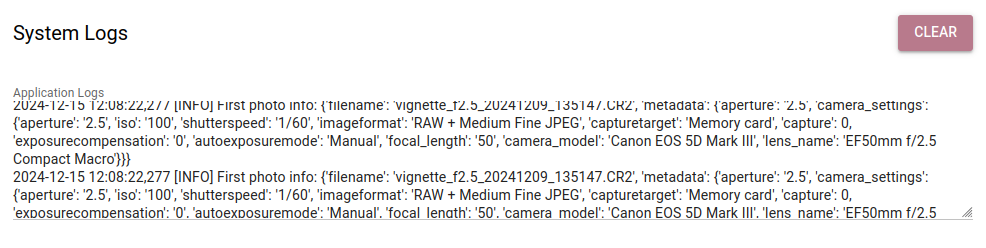
\includegraphics[width=1\textwidth]{Images/system_logs.png}
\caption{System logs.}
\label{fig:ui_system_logs}
\end{figure}

\subsection{Notifications}

The notification system provides real-time feedback to users. Notifications appear dynamically within the user interface to report critical events, such as successful camera connections and image captures. They also alert users to errors, including connection failures, invalid configurations, or file transfer issues.

\begin{figure}[h]
\centering

\includegraphics[width=0.7\textwidth]{Images/notification.png}
\caption{Notification example.}
\label{fig:ui_notification}
\end{figure}

\subsection{Additional Features}

The application includes several key features that enhance user experience and functionality. It can operate fully offline after the initial installation, allowing users to utilize its features without internet connectivity. A dark mode option is available, improving usability in low-light environments and providing a more comfortable viewing experience. Additionally, the application stores user interface state, including user preferences and currently opened elements, between visits, ensuring a seamless and consistent user experience.

\section{Testing}

To ensure the reliability and correctness of the application, particularly in the context of the "garage lab" approach described in the methodology, we implemented a comprehensive test suite using the pytest framework. The tests were designed to validate both the technical functionality and the practical usability of the application.

\subsection{Test Architecture}

Our test suite is organized into four main components, reflecting the modular architecture of the application. We divided the tests among \texttt{test\_camera\_manager.py}, which validates camera control and image acquisition; \texttt{test\_dataset\_manager.py}, which ensures proper data organization and persistence; \texttt{test\_analysis.py}, which verifies image processing and lens measurement algorithms; and \texttt{test\_ui.py}, which tests user interface components and interactions.

\subsection{Camera Manager Tests}

Tests for the Camera Manager focus on ensuring reliable camera operation across various scenarios. They evaluate the initialization process and connection management, verify the accuracy and consistency of image capture and metadata extraction, and test the configuration of the camera for different testing scenarios. Additionally, these tests assess the processing of EXIF data to extract detailed lens information and evaluate the effectiveness of error handling and recovery mechanisms.

\subsection{Dataset Manager Tests}

Dataset Manager tests evaluate the core functionalities of the \texttt{DatasetManager} class, ensuring proper management of datasets and their associated scenarios. These tests verify the creation, listing, updating, and deletion of datasets, as well as the addition and modification of scenarios within datasets. Additionally, they assess the export and import capabilities to confirm that datasets are correctly archived and restored with all metadata and content.

\subsection{Analysis Tests}

The analysis tests validate various functionalities of the lens measurement algorithms, ensuring accurate evaluation of lens properties. The tests cover sharpness analysis, distortion measurement, vignetting detection, chromatic aberration evaluation, and bokeh analysis. They verify methods for detecting edges, calculating modulation transfer functions (MTF), analyzing visual artifacts, and generating visualizations. Additionally, tests for preprocessing RAW images, feature extraction, and score calculation for lens performance are included.

\subsection{UI Tests}

UI tests focus on ensuring the functionality, responsiveness, and reliability of the user interface in managing camera operations, datasets, and scenarios. These tests validate the integration of UI components with backend functionality, covering critical workflows such as camera connection, configuration, photo capture, and metadata visualization. They assess the behavior of UI elements like buttons, dialogs, and status indicators under different conditions, including error states. Furthermore, the tests verify that key user actions, such as dataset and scenario creation, RAW file import, and analysis result display, operate seamlessly. Mocked components are used to simulate interactions, ensuring the interface effectively handles real-world scenarios and unexpected events.

\subsection{Test Fixtures and Mocking}

To facilitate reliable software testing within the "garage lab" approach, the test suite employs a range of fixtures and mocking techniques. Key test fixtures include \texttt{mock\_camera}, which simulates camera behavior; \texttt{mock\_camera\_manager}, which provides camera control testing; \texttt{temp\_dir}, which manages test file storage; \texttt{dataset\_manager}, which handles test data organization; and \texttt{sample\_image}, which provides standardized test images.

External dependencies, such as camera operations and file system interactions, are mocked to ensure consistency and reproducibility. Similarly, UI components are simulated to validate user interactions, while image processing operations rely on controlled test data to maintain accuracy and isolate external influences. These strategies enable thorough and reliable testing in a constrained, repeatable environment.

\subsection{Quality Assurance}

The test suite ensures quality assurance across multiple dimensions to verify the robustness and reliability of the application.

Functional testing evaluates the core features, such as the reliability of camera control, accuracy of data management, precision of analysis algorithms, and responsiveness of the user interface.

Error handling is assessed by simulating common issues, including camera connection failures, invalid user inputs, resource constraints, and potential data corruption, to ensure graceful recovery and system stability.

Performance testing examines the efficiency of image processing algorithms and memory usage optimization, measures application response times, and confirms that resources are effectively cleaned up after operations.

Together, these tests provide a comprehensive framework to validate the functionality, reliability, and performance of the application under diverse conditions. Test coverage reports are generated using pytest-cov to ensure thorough testing of all components, with particular attention to critical paths in the lens measurement workflows.

\section{Dataset Management Architecture}

Managing lens testing datasets effectively involves making strategic architectural choices. Two distinct approaches were considered: a centralized server-side management approach and a split browser-server model. Each approach offers different advantages and tradeoffs that were evaluated against the application's specific requirements.

\subsection{Approach Comparison}

\subsubsection{Centralized Server-Side Management}

The centralized server-side management approach involves maintaining all dataset management on the server, including both metadata and RAW files. This approach offers several advantages. It ensures strong data consistency with a single source of truth, simplifies transaction management for dataset operations, and reduces complexity in maintaining data synchronization. It is also better suited for multi-user scenarios and facilitates easier backup and version control of complete datasets. However, this approach has its disadvantages, such as higher server resource utilization, increased network traffic for metadata operations, potential latency in UI operations, and a less responsive interface for dataset organization.

\subsubsection{Split Browser-Server Management}

The split browser-server management approach divides responsibilities by handling metadata management in the browser while RAW files remain on the server. This leads to a more responsive user interface for dataset operations, reduces server load for metadata tasks, and lowers bandwidth usage for organizational activities. Additionally, it enhances offline capabilities for dataset organization and allows faster sorting and filtering of datasets. On the downside, this approach introduces more complex data synchronization requirements, potential consistency issues between client and server, and adds complexity in handling multi-user scenarios. It also complicates error recovery and necessitates conflict resolution in metadata.

\subsection{Technical Considerations}

Several technical aspects were considered when evaluating these approaches, including data storage, network usage, scalability, implementation complexity, and error handling. Centralized management involves managing all data in the server filesystem and database, resulting in higher network usage for metadata operations but consistent handling for RAW files. It is limited by server resources and has lower implementation complexity, being a straightforward Python implementation. Error handling is simpler, with easier recovery from failures.

In contrast, split management stores RAW files on the server and metadata in browser storage, resulting in lower network usage for metadata but the same for RAW files. It offers better scalability through distributed computational load but has higher implementation complexity due to the need for browser-server synchronization. Error handling is more complex, requiring more sophisticated state management.

\begin{table}[h]
\centering
\begin{tabular}{|p{3cm}|p{5cm}|p{5cm}|}
\hline
\textbf{Aspect} & \textbf{Centralized} & \textbf{Split Management} \\
\hline
Data Storage & All data managed in server filesystem and database & RAW files on server, metadata in browser storage \\
\hline
Network Usage & Higher for metadata operations, consistent for RAW files & Lower for metadata, same for RAW files \\
\hline
Scalability & Limited by server resources & Better distribution of computational load \\
\hline
Implementation Complexity & Lower, straightforward Python implementation & Higher, requires browser-server synchronization \\
\hline
Error Handling & Simpler recovery from failures & More complex state management required \\
\hline
\end{tabular}
\caption{Technical Comparison of Dataset Management Approaches}
\label{table:dataset_comparison}
\end{table}

\subsection{Selected Approach}

For this implementation, the centralized server-side management approach was chosen for several key reasons. The critical nature of lens testing data requires strong consistency guarantees, which are best provided by a single source of truth. The simpler architecture allows for faster development and testing, adhering to the project's implementation timeline. Additionally, this approach provides a better foundation for future expandability, such as adding multi-user support and version control. Maintaining data integrity is easier with centralized management, as it simplifies referential integrity between metadata and RAW files. Moreover, error recovery is more straightforward, with simpler backup and recovery procedures.

While the split browser-server model offers advantages in UI responsiveness and resource distribution, the added complexity and potential consistency issues were deemed to outweigh these benefits for the current scope of the application. However, the architecture remains modular enough that transitioning to a split model could be implemented in future versions if requirements change.

The selected architecture aligns well with the project's primary goals of reliability and accuracy in lens testing, maintaining a balance between implementation complexity and system robustness.

\section{Analysis Results Architecture}

Storing and managing analysis results for lens tests required careful architectural consideration. Two approaches were evaluated: embedded results and separate results storage.

\subsection{Approach Comparison}

\subsubsection{Embedded Results}

The embedded results approach involves storing analysis results directly with photo metadata. This method offers several advantages, including a simpler data structure and direct access to results without the need for separate storage management. It also facilitates easier data export since results are integrated with the images. However, this approach has its drawbacks, such as increased metadata size, reduced flexibility for multiple analyses, and potential performance impacts on metadata operations due to the larger data volumes.

\subsubsection{Separate Results Storage}

The separate results storage approach manages analysis results in distinct storage structures, separate from photo metadata. This offers greater flexibility in managing analyses, improved performance for handling large datasets, easier implementation of result versioning, and independent scaling of storage resources. On the downside, it introduces more complex data relationships, requires additional storage management, and can lead to potential consistency challenges between results and the corresponding images.

\subsection{Selected Approach}

For this implementation, the embedded results approach was chosen due to its simplicity and direct alignment with the project's scope. By storing analysis results alongside photo metadata, the system maintains a straightforward data structure and facilitates easier data export processes. Although this approach has some limitations, such as increased metadata size, it meets the current requirements effectively. The architecture allows for future transitions to separate storage if the need arises, ensuring scalability and flexibility for future developments.

\section{Camera Control Architecture}

Designing the camera control systems involved a fundamental architectural decision: whether to use direct library integration via gphoto2 or to implement a REST API-based control system. Both approaches have distinct characteristics that influence the application's functionality and maintainability.

\subsection{Approach Comparison}

\subsubsection{Direct gphoto2 Integration}

Direct integration with the gphoto2 library through Python bindings was selected for this application. This approach offers several advantages, including lower latency for camera operations and direct access to all camera features. It simplifies error handling by allowing direct exception propagation and eliminates the need for an additional network stack. Handling large RAW file transfers is more efficient, and full access to real-time camera events is possible. However, this approach results in tight coupling to the gphoto2 library, has platform-dependent installation requirements, and involves a more complex deployment process. It is also limited to local camera connections and subject to version compatibility constraints.

\subsubsection{REST API-based Control}

The alternative approach involves implementing a REST API layer for camera control. This offers platform-independent operation and easier integration with other systems. It supports remote camera control and simplifies deployment through containerization. The REST API-based approach promotes better separation of concerns and allows for load balancing. Nevertheless, it introduces additional network latency, complicates error handling, and adds overhead due to the HTTP protocol. Managing API versions and ensuring network security also adds to the complexity.

\subsection{Technical Considerations}

The technical differences between the two approaches are significant. Direct integration offers minimal latency and direct memory access, leading to higher performance in camera operations. Deployment requires installing the gphoto2 library, which can be complex, but the system can handle large RAW file transfers more efficiently. Security relies on system-level permissions. Scalability is limited to local connections, and error handling involves direct exception propagation.

In contrast, the REST API approach introduces network-dependent latency and relies on HTTP for communication, which can impact performance. Deployment is more straightforward and container-friendly, enhancing portability. Security requires managing network security, and scalability is improved through support for distributed systems. Error handling involves HTTP status codes and messages, adding layers of complexity.

\begin{table}[h]
\centering
\begin{tabular}{|p{3cm}|p{5cm}|p{5cm}|}
\hline
\textbf{Aspect} & \textbf{Direct Integration} & \textbf{REST API} \\
\hline
Performance & Minimal latency, direct memory access & Network-dependent latency \\
\hline
Deployment & Requires library installation & Container-friendly, portable \\
\hline
Security & System-level permissions & Network security required \\
\hline
Scalability & Limited to local connections & Supports distributed systems \\
\hline
Error Handling & Direct exception propagation & HTTP status codes and messages \\
\hline
\end{tabular}
\caption{Technical Comparison of Camera Control Approaches}
\label{table:camera_control_comparison}
\end{table}

\subsection{Implementation Impact}

Choosing the direct integration approach impacts implementation significantly. For example, capturing an image using direct integration involves straightforward method calls with exception handling:

\begin{verbatim}
def capture_image(self):
    try:
        file_path = self.camera.capture(gp.GP_CAPTURE_IMAGE)
        camera_file = self.camera.file_get(
            file_path.folder,
            file_path.name,
            gp.GP_FILE_TYPE_NORMAL
        )
        return camera_file
    except gp.GPhoto2Error as e:
        logging.error(f"Capture failed: {e}")
        raise
\end{verbatim}

In contrast, a REST API-based implementation would require setting up HTTP endpoints and handling responses accordingly:

\begin{verbatim}
@app.post("/api/camera/capture")
async def capture_image():
    try:
        response = await client.post(
            f"{CAMERA_SERVICE_URL}/capture",
            headers={"Authorization": AUTH_TOKEN}
        )
        if response.status_code == 200:
            return response.json()
        raise HTTPException(status_code=response.status_code)
    except Exception as e:
        raise HTTPException(status_code=500, detail=str(e))
\end{verbatim}

\subsection{Selected Approach}

The direct gphoto2 integration approach was chosen for this application due to several key factors. Performance was a priority, requiring minimal latency for precise timing of captures and settings changes. Direct access to camera events was crucial for monitoring camera status and capture completion in real-time. Handling large RAW files efficiently was necessary, and direct exception handling provided better control over camera-related errors. Additionally, full access to camera features without API abstraction limitations was essential for comprehensive camera control.

While the REST API-based approach offers advantages in scalability and system integration, the performance and control requirements of lens testing necessitated the direct integration approach. The tight coupling to gphoto2 is managed through careful abstraction in the \texttt{CameraManager} class, allowing for potential future adaptations if requirements change.

\subsection{Future Considerations}

\subsubsection{Application Workflow}

The application follows a straightforward capture-and-analyze workflow. Upon opening the application, the user is presented with the camera control panel to connect their camera. After successfully connecting, the user can proceed with lens testing by selecting a scenario, such as vignetting or bokeh, from the scenarios panel. Each scenario comes with predefined settings optimized for that specific test.

Next, the user initiates the capture phase by clicking the capture button, which opens an aperture selection dialog. Here, multiple aperture values can be selected for comparison—such as f/1.8, f/2.8, and f/4—to observe how vignetting changes with aperture. Upon confirming the aperture selections, the system automatically captures images at each selected aperture value.

The captured images are displayed in a scrollable list view, each showing a thumbnail preview and capture settings. The system processes these images sequentially, running the analysis algorithms specific to the chosen scenario.

As analysis completes for each image, the results are displayed in the analysis panel. Users can click on any analyzed image to view detailed results, including measurements, visualizations, and comparisons across different apertures. This workflow can be repeated for each scenario the user wishes to test. All results are automatically saved within the dataset, allowing users to revisit them later or export them for sharing.

\subsubsection{Metadata Collection Implementation}

The system implements a dual-source approach to metadata collection by combining EXIF data extraction with direct gphoto2 camera queries. This redundancy was necessary due to significant reliability issues encountered with both sources.

EXIF metadata extraction often produced inconsistent results because manufacturer-specific implementations stored critical lens data in varying tags or formats. For example, focal length information might appear in multiple fields with conflicting values, or lens identification could be split across several tags. Some cameras omitted crucial metadata entirely, while others populated fields with incorrect values.

The gphoto2 interface, while providing direct camera access, also presented challenges. Camera responses to property queries were unpredictable, varying between manufacturers and even between firmware versions of the same model. Some cameras would temporarily lock up when queried for certain properties, requiring timeout handling and retry logic.

To address these issues, the implementation includes cross-validation between EXIF and gphoto2 data, manufacturer-specific parsing rules for common cameras, fallback mechanisms for critical properties through user input, and aggressive timeout handling for camera queries. The system maintains a mapping of known metadata inconsistencies and their workarounds, which will grow as more camera models are supported.

This dual-source approach, while more complex than relying on a single metadata source, ensures the reliability needed for accurate lens testing. However, it remains one of the more fragile aspects of the system, requiring regular updates as new cameras and firmware versions introduce different metadata handling behaviors.

\subsection{PTP Communication Layer}

Camera communication relies on the Picture Transfer Protocol (PTP) through the gphoto2 library. PTP is a standardized protocol for digital imaging devices, intended to provide a consistent interface across different camera manufacturers. However, the implementation revealed several practical challenges.

While PTP specifies standard operations for camera control and image transfer, manufacturers often implement vendor-specific extensions. For example, Canon's PTP implementation includes proprietary commands for live view and advanced settings control, whereas Nikon uses different command sets for similar features. This fragmentation necessitated implementing manufacturer-specific code paths for certain operations.

The protocol's reliability varied significantly across different scenarios. Some cameras would disconnect during long operations, bulk transfers occasionally failed without error signals, certain commands could cause camera lockups, and response timeouts varied unpredictably.

To mitigate these issues, a robust PTP/gphoto2 session management system was implemented. This system monitors connection health, automatically recovers from protocol errors, and maintains session state. Additionally, command retry logic was introduced to handle temporary communication failures.

While the gphoto2 library abstracts much of the low-level PTP complexity, understanding the protocol's limitations was essential for building reliable camera control. For instance, the system avoids sending rapid sequences of PTP commands that might overwhelm camera buffers and includes error handling for known protocol edge cases.

\subsection{Containerized Operation}

The application supports containerized deployment for scenarios where camera control isn't needed, such as reviewing existing datasets or performing analysis on previously captured images. This deployment uses Docker to create an isolated environment with all required dependencies.

The container configuration excludes the gphoto2 library, as physical camera access isn't necessary. This reduces the container size and simplifies cross-platform deployment. The container includes only the core analysis components and dataset management functionality.

\begin{figure}[h]
\centering
\includegraphics[width=0.8\textwidth]{Images/docker_architecture.png}
\caption{Docker deployment architecture.}
\label{fig:docker_architecture}
\end{figure}

The containerized version maintains the same dataset structure and analysis capabilities as the full application. Users can import existing datasets, perform analysis, and export results. The key difference is that new image capture isn't possible— all operations work with pre-existing or imported RAW files.

Data persistence is handled through volume mounting, allowing datasets to be stored outside the container. This enables easy backup and sharing of datasets between container instances:

\begin{verbatim}
docker run -v /path/to/datasets:/app/datasets -p 8080:8080 clona
\end{verbatim}

The containerized deployment provides a way to run the application's analysis features without dealing with camera hardware dependencies. This is useful in educational settings or when reviewing results on systems without camera connectivity.
